\chapter{Reinforcement learning}
\label{cha:reinforcement}

The main character of a reinforcement learning setting is an \textit{agent},
usually referred to in the slide as the \textit{learner}. The learner interacts
with an environment by means of actions. At any given point of time $t$, the
learner is in a state $s_{t}$ which belongs to a set of possible states
$\mathcal{S}$. For each state $s_{t} \in \mathcal{S}$ the learner can perform a set
of possible actions $a_{t} \in \mathcal{A}$ in order to move to a next state $s_{t+1}$.
In performing action $a$ from state $s$, the learner is provided an immediate \textit{reward}
$r(s,a)$ (possibly negative). The behaviour of the agent is regulated by a \textit{policy
function} $\pi: \mathcal{S}\rightarrow \mathcal{A}$. The task of a reinforcement
learning algorithm is to learn a policy allowing to choose for each state $s$ the
action $a$ maximizing the overall reward. A high level graphical representation
of this learning setting is depicted in Figure \ref{fig:reinforcementLearning}.
\newline

The typical challenges faced by the leaner during this process are:
\begin{itemize}
	\item \textit{delayed reward} coming from future moves

	\item trade-off between \textit{exploitation} and \textit{exploration}
\end{itemize}

\begin{figure}[H]
	\centering
	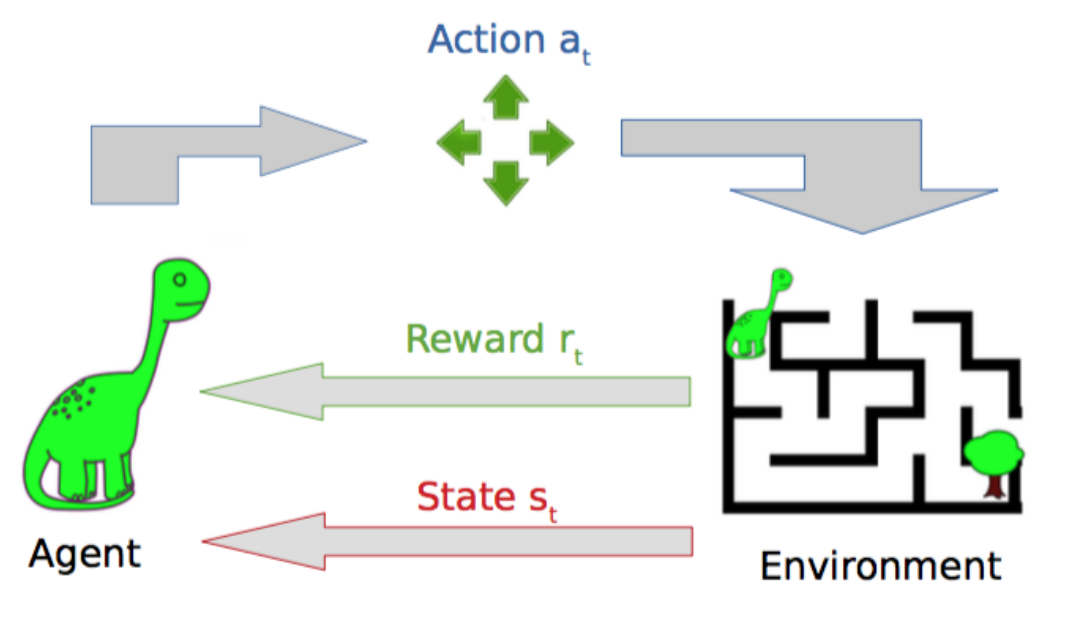
\includegraphics[width=0.72\textwidth]{
		images/19_ReinforcementLearning_reinforcementLearning.png
	}
	\caption{High level idea of a reinforcement learning setting}
	\label{fig:reinforcementLearning}
\end{figure}

\section{Applications}
Reinforcement learning has several real world applications. The main research
fields where reinforcement learning solutions are adopted are:

\begin{itemize}
	\item videogames:
		\begin{itemize}
			\item objective = complete the game with the highest score

			\item state = raw pixel inputs of the game state

			\item action = game controls (left, right, up, down)

			\item reward = score increase/decrease
		\end{itemize}

	\item robotics

	\item board games (e.g. Go):
		\begin{itemize}
			\item objective = win the game

			\item state = position of all pieces

			\item action = where to put the next piece down

			\item reward = 1 if win at the end of the game, 0 otherwise
		\end{itemize}
\end{itemize}

\section{Markov Decision Process MDP}
\textit{Markov Decision Process} (MDP) is a framework used to help to make
decision on a \textit{stochastic environment}. In a stochastic environment there
is uncertainty in the result of a decision.\\ Formally a MDP is defined by a
tuple of five elements: ($\mathcal{S}, \mathcal{A}, \mathcal{R}, \mathcal{P}, \gamma$):
\begin{itemize}
	\item a set of states $\mathcal{S}$ in which the agent can be at each time instant.
		At the beginning the learner is at the initial state $s_{0}$. In $S$ there is
		a (possibly empty) set of \textit{teminal states}
		$\mathcal{S}_{G} \subset \mathcal{S}$

	\item a set of actions $\mathcal{A}$ the agent can make

	\item a reward function $R(s,a,s')$ for making action $a$ in state $s$ and reaching
		state $s'$

	\item a \textit{transition} model providing the probability of going to a
		state $s'$ with action $a$ from state $s$. \textit{Markov assumption} is
		that the probability of going to $s'$ from $s$ depends only on $s$ and not
		on any other past actions or states.
		\begin{equation}
			P(s'|s,a) \; s,s' \in \mathcal{S}, a \in \mathcal{A}
		\end{equation}

	\item \textit{discount factor} $\gamma$: a scalar (optional)
\end{itemize}

In Figure \ref{fig:mdpExample} there is illustrated an example of MDP. In this
case, we have an agent moving in a room. The elements of the MDP are:
\begin{itemize}
	\item state = occupied cell

	\item terminal states (row, column) = (4,2), (4,3)

	\item actions = UP, DOWN, LEFT, RIGHT

	\item transitions probabilities = 0.8 in direction of action, 0.1 in each
		orthogonal direction

	\item rewards = $R((4,2)) = -1$, $R((4,3)) = +1$
\end{itemize}

\begin{figure}[H]
	\centering
	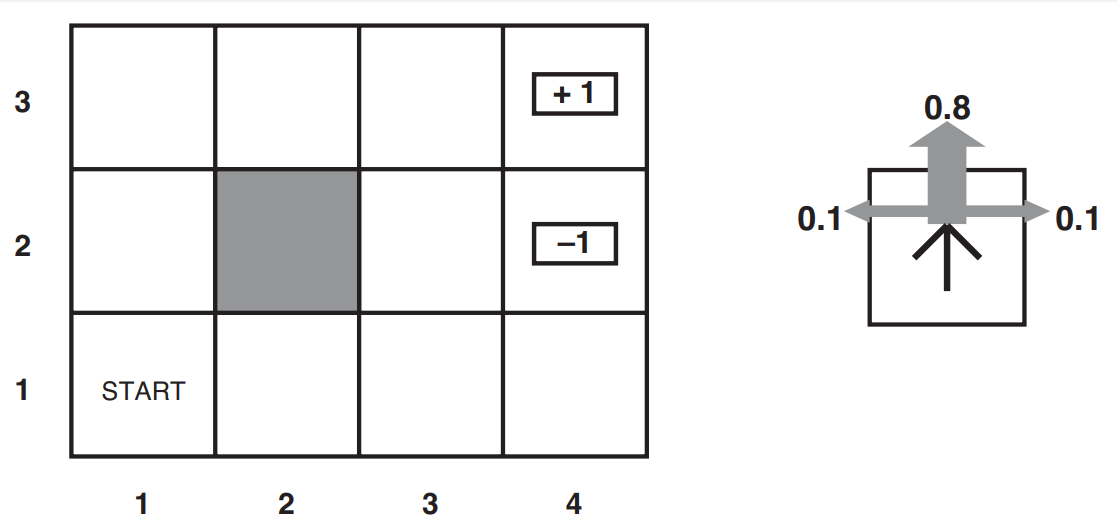
\includegraphics[width=\textwidth]{
		images/19_ReinforcementLearning_markovDecisionProcess.png
	}
	\caption{MDP Example}
	\label{fig:mdpExample}
\end{figure}

An \textit{environment history} is a sequence of states. For example, a certain
policy $\pi$ starting in state $s_{0}$ could lead to a sequence of states
$s_{0}, s_{1}, s_{2}, \hdots$. \textit{Utilities} are defined over environment
histories. In the following of the section we are going to take into account the
following assumptions:
\begin{itemize}
	\item we assume an \textit{infinite horizon} (no constraints on the number of time
		steps)

	\item we assume \textit{stationary} preferences, i.e. if one history is
		preferred to another at time $t$, the same should hold at time $t'$ provided
		they start from the same state
\end{itemize}

Given an environment history $s_{0}, s_{1}, s_{2}, \hdots$, the utility can be
computed in two main ways:
\begin{itemize}
	\item \textit{additive rewards}
		\begin{equation}
			U([s_{0}, s_{1}, s_{2}, \hdots]) = R(s_{0}) + R(s_{1}) + R(s_{2}) + \hdots
		\end{equation}

	\item \textit{discounted rewards}
		\begin{equation}
			U([s_{0}, s_{1}, s_{2}, \hdots]) = R(s_{0}) + \gamma R(s_{1}) + \gamma^{2}
			R(s_{2}) + \hdots
		\end{equation}
\end{itemize}

\textbf{Remark:} in the more general case each reward should be written as $R(s_{t}
, a_{t}, s_{t+1})$
\newline

\textbf{Remark:} the lower the discount factor $\gamma$ is, the less important
future rewards are, and the agent will tend to focus on actions which will yield
immediate rewards only.

\subsection{Taking decisions}
A \textit{policy} $\pi$ is a full specification of what action to take at each
state.
\newline

The \textit{expected utility} of a policy is the utility of an environment history,
taken in expectation over all possible histories generated with that policy.
\newline

An \textit{optimal policy} $\pi*$ is a policy maximizing expected utility. In
Figure \ref{fig:optimalPolicy} we propose an example of optimal policy:
\begin{itemize}
	\item utility is made with additive rewards

	\item $r$ is the reward of non-terminal states

	\item arrows indicate the best action to take

	\item star indicates all actions are equally optimal
\end{itemize}
From the proposed structure we can make the following observations:
\begin{itemize}
	\item if moving is very expensive, optimal policy is to reach any terminal
		state as soon as possible

	\item if moving is very cheap, optimal policy is avoiding the bad terminal
		state at all costs

	\item if moving gives positive reward, optimal policy is to stay away of
		terminal states
\end{itemize}

\textbf{Remark:} for infinite horizons, optimal policies are \textit{stationary},
i.e. they only depend on the current state.

\begin{figure}[H]
	\centering
	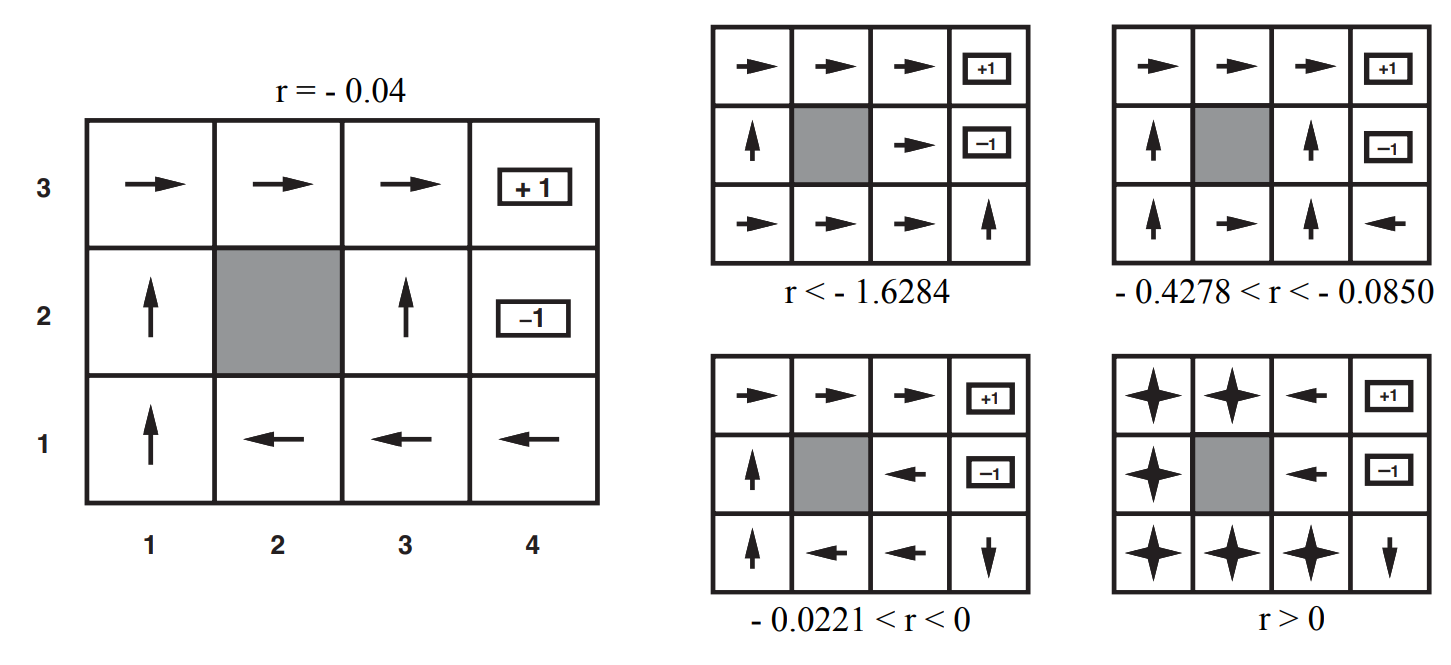
\includegraphics[width=0.85\textwidth]{
		images/19_ReinforcementLearning_optimalPolicy.png
	}
	\caption{Optimal policy example}
	\label{fig:optimalPolicy}
\end{figure}

\section{Learning the optimal policy}
As opposed to supervised learning methods, in reinforcement learning, the learning
loop does not allow us to define a loss function directly. As a result the
learning procedure is more complicated. In general the solution is to let the agent
exploring the environment and update the policy according to the achieved reward.
More in depth, the literature proposes two main learning approaches:
\begin{itemize}
	\item \textbf{value-based methods:}
		\begin{itemize}
			\item the goal of the agent is to optimize the utility of a state $U(s)$ which
				quantifies "how good" is a state

			\item the value of each state $s$ is the total amount of the reward an agent
				can expect to collect over the future from $s$

			\item maximizing $U(s)$ for each state, we indirectly optimize the policy
		\end{itemize}

	\item \textbf{policy base methods}: we define a policy which we need to optimize
		directly. To do this, we typically learn a neural network which outputs a \textit{stochastic
		policy}, i.e. a probability distribution over different actions.
		\[
			\pi_{\theta} (s,a) \approx P(a|s)
		\]
\end{itemize}

\subsection{Value based methods}
The utility function gives the total amount of reward the agent can expect from a
particular state to all possible state from that state. With the utility
function we are going to find a policy. More formally, the utility $U$ of a
state $s$ given a policy $\pi$ is the expected cumulative reward we can get
following policy $\pi$ starting from $s$:
\begin{equation}
	U^{\pi}(s) = E[\sum_{t=0}^{\infty}\gamma^{t} r(s_{t}) | s_{0} = s, \pi]
\end{equation}
with: $a_{t} = \pi(s_{t})$ ; $s_{t+1}\sim P(\cdot | s_{t}, a_{t})$
\newline

The true utility of a state is its utility under an optimal policy:
\begin{equation}
	U(s) = U^{\pi^{*}}(s) = \text{max}_{\pi}E[\sum_{t=0}^{\infty}\gamma^{t} r(s_{t}
	) | s_{0} = s, \pi]
\end{equation}
Given the true utility, an optimal policy is as follows:
\begin{equation}
	\pi^{*}(s) = \text{argmax}_{a \in \mathcal{A}}\sum_{s' \in \mathcal{S}}p(s' | s
	, a) U(s')
\end{equation}

For each state $s \in S$ we define a \textbf{Bellman equation}: \textit{the
utility of a state is its immediate reward plus the expected discounted utility
of the next state, assuming that the agent chooses an optimal action}.
\begin{equation}
	U(s) = R(s) + \gamma * \text{max}_{a \in \mathcal{A}}\sum_{s' \in S}p(s' | s,a)
	U(s')
\end{equation}
Utilities of states are solutions of the set of Bellman equations. The solutions
to the set of Bellman equations are unique. However, directly solving the set of
equations is hard. As a consequence, we rely on a dynamic programming
algorithmic approach (\textit{value iteration}):
\begin{itemize}
	\item \textbf{step 1:} initialize $U_{0}(s)$ to zero for all $s$

	\item \textbf{step 2:} repeat until max utility difference is below a
		threshold
		\begin{itemize}
			\item \textbf{step 2.1:} do Bellman update for each state $s$:
				\[
					U_{i+1}(s) \leftarrow R(s) + \gamma * \text{max}_{a \in \mathcal{A}}\sum
					_{s' \in \mathcal{S}}p(s'|s,a)U_{i}(s')
				\]

			\item \textbf{step 2.2:} $i \leftarrow i+1$
		\end{itemize}

	\item \textbf{step 3:} return $U$
\end{itemize}

This latter algorithm is used as a subroutine of the following algorithm (\textit{policy
iteration}) which is used to learn the optimal policy:
\begin{itemize}
	\item \textbf{step 1:} initialize $\pi_{0}$ randomly

	\item \textbf{step 2:} repeat until no policy improvement
		\begin{itemize}
			\item \textbf{step 2.1: policy evaluation} solve set of linear equations (as
				explained in the previous algorithm):
				\[
					U_{i}(s) = R(s) + \gamma \sum_{s' \in \mathcal{S}}p(s' | s, \pi_{i}(s))
					U_{i}(s') \; \forall s \in \mathcal{S}
				\]
				where $\pi_{i}(s)$ is the action that policy $\pi_{i}$ prescribes for state
				$s$

			\item \textbf{step 2.2: policy improvement}
				\[
					\pi_{i+1}(s) \leftarrow \text{argmax}_{a \in \mathcal{A}}\sum_{s' \in \mathcal{S}}
					p(s'|s,a)U_{i}(s') \; \forall s \in \mathcal{S}
				\]

			\item \textbf{step 2.3:} $i \leftarrow i+1$
		\end{itemize}

	\item \textbf{step 3:} return $\pi$
\end{itemize}

\section{Reinforcement learning in an unknown environment}

Value iteration and policy iteration assume perfect knowledge (environment, transition
model, rewards). However, in most cases, some of these aspects are not known. In
order to face this limitation, reinforcement learning aims at learning policies
by space exploration.
\begin{itemize}
	\item \textbf{policy evaluation:} the policy is given and the passive agent
		explores the environment

	\item \textbf{policy improvement:} the policy is learnt while the active agent
		explores the environment
\end{itemize}

\subsection{Adaptive Dynamic Programming (ADP) algorithm}
In this case we assume that the environment is unknown and that the policy is
given. The fact that we don't know the environment means that we don't know the states,
the transitions probabilities and so on. The idea in this case is to explore the
space collecting rewards $r$ and saving them as a reward function $R(s)=r$. Then
we take the action given by the policy (that is given) bringing the agent to
state $s'$. Now we update the counts that allows to compute the transition probability
function $p$ incrementing by one the number of times we are in state $s$ and we take
action $a$, i.e.
\begin{equation}
	N_{sa}\leftarrow N_{sa}+1
\end{equation}

In addition we keep track of the number of times we are in state $s$ and take an
action $a$ brings the agent to state $s'$:
\begin{equation}
	N_{s'|sa}\leftarrow N_{s'|sa}+1
\end{equation}

At this point we have all the information that we need to update the transition
model, by using maximum likelihood estimation. The probability of reaching state
$s''$ being in state $s$ taking action $a$ is given by the fraction of times in
which the agent is in state $s$ and take an action $a$ that brings the agent to
state $s''$ divided by the number of times we are in state $s$ and we take
action $a$:
\begin{equation}
	p(s''|s,a) = \frac{N_{s''|sa}}{N_{sa}}\; \forall s'' \in \mathcal{S}
\end{equation}

The last step is to run \textit{policy-evaluation} to obtain the utility estimate
$U$ ($U$ is initially empty). Each step is expensive as it runs policy
evaluation.

\begin{itemize}
	\item \textbf{step 1:} initialize $s$

	\item \textbf{step 2:} repeat until $s$ is terminal
		\begin{itemize}
			\item \textbf{step 2.1:} receive reward $r$, set $R(s) = r$

			\item \textbf{step 2.2:} choose next action $a \leftarrow \pi(s)$

			\item \textbf{step 2.3:} take action $a$, reach step $s'$

			\item \textbf{step 2.4:} update counts
				\[
					N_{sa}\leftarrow N_{sa}+1
				\]
				\[
					N_{s' | sa}\leftarrow N_{s' | sa}+1
				\]

			\item \textbf{step 2.5:} update transition model
				$\forall s'' \in \mathcal{S}$
				\[
					p(s'' | s,a) \leftarrow \frac{N_{s''|sa}}{N_{sa}}
				\]

			\item \textbf{step 2.6:} update utility estimate
				\[
					U \leftarrow \text{policyEvaluation}(\pi, U, p, R, \gamma)
				\]
		\end{itemize}
\end{itemize}

\subsection{Temporal-difference (TD) policy evaluation}
This is an approximate method that avoids to run policy evaluation at each iteration
to compute the correct utility (expensive). The algorithms instead approximates
the utility of the state which is based on the intuition that if we are in state
$s$ and the policy suggests to take action $a$ and reach $s'$, then if $s'$ was \textit{always}
the successor of $s$ the utility of $s$ should be computed as:
\begin{equation}
	U(s) = R(s) + \gamma U(s')
\end{equation}
Note that this is a rough approximation, not the exact utility of the state $s$.\\
Now the idea is to try to make the utility closer to the above approximation. Making
the current $U(s)$ closer to $R(s)+ \gamma U(s')$ can be possible by updating the
current $U(s)$ in such a way that the difference between what we want ($R(s)+ \gamma
U(s')$) and what we have (the current $U(s)$)
\begin{equation}
	U(s) = U(s) + \alpha(R(s) + \gamma U(s') - U(s))
\end{equation}
where $\alpha$ is a learning rate (possibly decreasing over time).
\newline

\textbf{Remark:} Note that we do not need a perfect estimate of the utility $U$
of the states, the only think that we want is a good utility of the states that allows
to find the best policy.
\newline

\textbf{Remark:} One of the main benefits of this algorithm is that it does not
need a transition model to update the utility. As a consequence, each step is
much faster than ADP. However, depending on the learning rate $\alpha$, TD policy
evaluation algorithm takes longer to converge. In a sense, this algorithm can be
seen as a rough efficient approximation of ADP.
\newline

\begin{itemize}
	\item \textbf{step 1:} initialize $s$

	\item \textbf{step 2:} repeat until $s$ is terminal
		\begin{itemize}
			\item \textbf{step 2.1:} receive reward $r$

			\item \textbf{step 2.2:} choose next action $a \leftarrow \pi(s)$

			\item \textbf{step 2.3:} take action $a$, reach step $s'$

			\item \textbf{step 2.4:} update local utility estimate
				\[
					U(s) \leftarrow U(s) + \alpha(r+\gamma U(s') - U(s))
				\]
		\end{itemize}
\end{itemize}

\subsection{Exploration vs exploitation trade-off}
Up to this point we know that policy learning requires combining learning the
environment and learning the optimal policy for the environment. Learning the environment
and performing policy evaluation (which requires solving system of linear
equations) are expensive tasks to accommodate. A simple trick is the one
followed by \textit{greedy agents}. The idea is to replace the policy evaluation
in ADP with optimal policy computation given the current knowledge of the
environment:
\begin{equation}
	U(s) = R(s) + \gamma \text{max}_{a \in \mathcal{A}}\sum_{s' \in \mathcal{S}}p(s
	' |s,a)U(s')
\end{equation}

The problem is that the knowledge of the environment is incomplete. As a consequence,
a greedy agent usually learns a suboptimal policy. More technically, this is a
result of lack of \textit{exploration}.
\newline

In Figure \ref{fig:greedyAgent} we propose an example of greedy agent behaviour.
The algorithm finds a policy reaching the +1 terminal state along the lower route
(2,1), (3,1), (3,2) and (3,3). It never learns the utilities of the other states.
As a result, it fails to discover the optimal route (1,2), (1,3) and (2,3).

\begin{figure}[H]
	\centering
	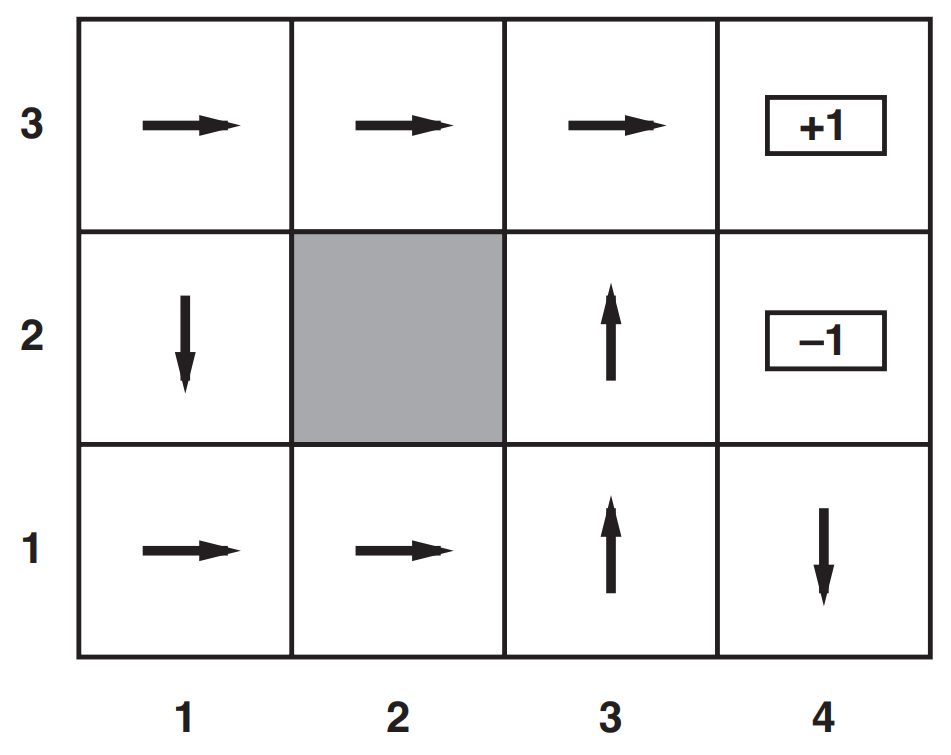
\includegraphics[width=0.7\textwidth]{
		images/19_ReinforcementLearning_greedyAgent.png
	}
	\caption{Greedy agent behaviour.}
	\label{fig:greedyAgent}
\end{figure}

The solution to face this problem is a good trade-off between \textit{exploitation}
and \textit{exploration}.
\begin{itemize}
	\item \textbf{Exploitation:} consists in following promising directions given
		current knowledge.

	\item \textbf{Exploration:} consists in trying novel directions looking for
		better (unknown) alternatives.
\end{itemize}

In order to find a good trade-off between the twos there are two approaches:
\begin{enumerate}
	\item $\epsilon$-greedy strategy: with probability $\epsilon$ the agent moves
		randomly (exploration) and with probability $1 - \epsilon$ goes greedy.

	\item another approach is to assign high utility estimates to unexplored state-action
		pairs and decrease the utility on an action if you already did it a lot of times,
		i.e. a high value of $N_{sa}$ causes the utility on that state to reduce.
\end{enumerate}

\begin{equation}
	U^{+}(s) = R(s) + \gamma \text{max}_{a \in \mathcal{A}}f(\sum_{s' \in \mathcal{S}}
	p(s' | s,a) U^{+}(s'), N_{sa})
\end{equation}
with $f$ increasing over the first argument and decreasing over the second.

\subsection{Q-learning}
As an alternative to what we have learnt so far, it is convenient to define the utility
of a state-action $(s,a)$ pair and not only of a state $s$. The value of a state-action
pair is written $Q(s,a)$. Given policy $\pi$, the utility of a state action pair
$(s,a)$ is computed as follows:
\begin{equation}
	Q^{\pi}(s,a) = E[\sum_{t=0}^{\infty}\gamma^{t} r(s_{t}) | s_{0} = s, a_{0} = a,
	\pi]
\end{equation}

The true utility of a state-action pair $(s,a)$ is its utility under an optimal
policy:
\begin{equation}
	Q(s,a) = Q^{\pi*}(s,a) = max_{\pi}E[\sum_{t=0}^{\infty}\gamma^{t} r(s_{t}) | s_{0}
	= s, a_{0} = a, \pi]
\end{equation}

Once $Q(s,a)$ has been computed for each state action pair, the optimal policy corresponds
to:
\begin{equation}
	\pi*(s) = \text{argmax}_{a \in \mathcal{A}}Q(s,a)
\end{equation}

The task is to progressively learn a table where we have the maximum expected future
reward, for each action at each state. As we are going to see in the next algorithmic
procedure, the update of the utility of a state action pair $(s,a)$ is again
computed by means of the Bellman equation:
\begin{equation}
	Q(s,a) = R(s) + \gamma \text{max}_{a \in \mathcal{A}}\sum_{s' \in \mathcal{S}}p
	(s'|s,a) U(s')
\end{equation}
The procedure is recursive:
\begin{itemize}
	\item \textbf{step 1:} initialize the $Q$ matrix with zeros

	\item \textbf{step 2:} select a random initial state and a discount factor

	\item \textbf{step 3:} for each \textit{episode} (set of actions that starts
		on the initial state and ends in the goal state)
		\begin{itemize}
			\item \textbf{step 3.1:} while state is not a goal state
				\begin{itemize}
					\item \textbf{step 3.1.1} select a random possible action for the
						current state

					\item \textbf{step 3.1.2} using this possible action consider going to
						this next state $s$

					\item \textbf{step 3.1.3} get maximum $Q$ value for this next state
						$s$ (taking into account all actions from this next state). This is computed
						solving Bellmann equation.
				\end{itemize}
		\end{itemize}
\end{itemize}

After some episode, my \textit{Q-table} encodes the optimal policy:
\begin{itemize}
	\item \textbf{step 1:} set current state = initial state

	\item \textbf{step 2:} repeat until current state = goal state

		\begin{itemize}
			\item \textbf{step 2.1:} from current state find the action with the
				highest $Q$ value

			\item \textbf{step 2.2:} set current state = next state (state from action
				chosen on step 2)
		\end{itemize}
\end{itemize}

This procedure assumes perfect knowledge of the environment, transition model, rewards.
However, this is not the case in most of the application. As a consequence we
can use ADP and TD algorithms also in this scenario. In particular TD SARSA algorithm
is implemented in this context as follows:

\begin{itemize}
	\item \textbf{step 1:} initialize $s$

	\item \textbf{step 2:} repeat until $s$ is terminal
		\begin{itemize}
			\item \textbf{step 2.1:} receive reward $r$

			\item \textbf{step 2.2:} choose next action
				$a \leftarrow \pi^{\epsilon}(s)$

			\item \textbf{step 2.3:} take action $a$, reach step $s'$

			\item \textbf{step 2.4:} choose action $a' \leftarrow \pi^{\epsilon}(s')$

			\item \textbf{step 2.5:} update local utility estimate
				\[
					Q(s,a) \leftarrow Q(s,a) + \alpha(r+ \gamma Q(s',a') - Q(s,a))
				\]
		\end{itemize}
\end{itemize}

This is an \textbf{on-policy} solution. On the other hand we introduce here an
alternative, referred to as \textit{Q-learning} which implements an \textbf{off-policy}
solution.

\begin{itemize}
	\item \textbf{step 1:} initialize $s$

	\item \textbf{step 2:} repeat until $s$ is terminal
		\begin{itemize}
			\item \textbf{step 2.1:} receive reward $r$

			\item \textbf{step 2.2:} choose next action
				$a \leftarrow \pi^{\epsilon}(s)$

			\item \textbf{step 2.3:} take action $a$, reach step $s'$

			\item \textbf{step 2.5:} update local utility estimate
				\[
					Q(s,a) \leftarrow Q(s,a) + \alpha(r+ \gamma \text{max}_{a' \in \mathcal{A}}
					Q(s',a') - Q(s,a))
				\]
		\end{itemize}
\end{itemize}

The main difference between SARSA and Q-learning is that SARSA is \textit{on-policy},
meaning that it updates $Q$ using the current policy's action. On the other hand
Q-learning is \textit{off-policy}, meaning that it updates $Q$ using the greedy policy's
action (which is NOT the policy it uses to search).
\newline

Off-policy methods are more flexible. On the other hand, on-policy methods tend to
converge faster, and are easier to use for continuous-state spaces and linear
function approximators about which we discuss in the following of this chapter.

\section{Scaling to large state spaces}
All techniques seen so far assume a tabular representation of utility functions
(e.g. state-action pairs). However, tabular representations do not scale to large
state spaces. For example Backgammon has an order of $10^{20}$ states.

\subsection{Function approximation}
The first solution to deal with this limitation is to rely on \textit{function
approximation} (Figure \ref{fig:functionApproximation}). In essence, our aim is to
approximate $U(s)$ or $Q(s,a)$ with a parametrized function. The function takes
a state representation as input. For example $(x,y)$ coordinates of a maze. With
this formulation, the function allows to generalize to unseen states.

\begin{figure}[H]
	\centering
	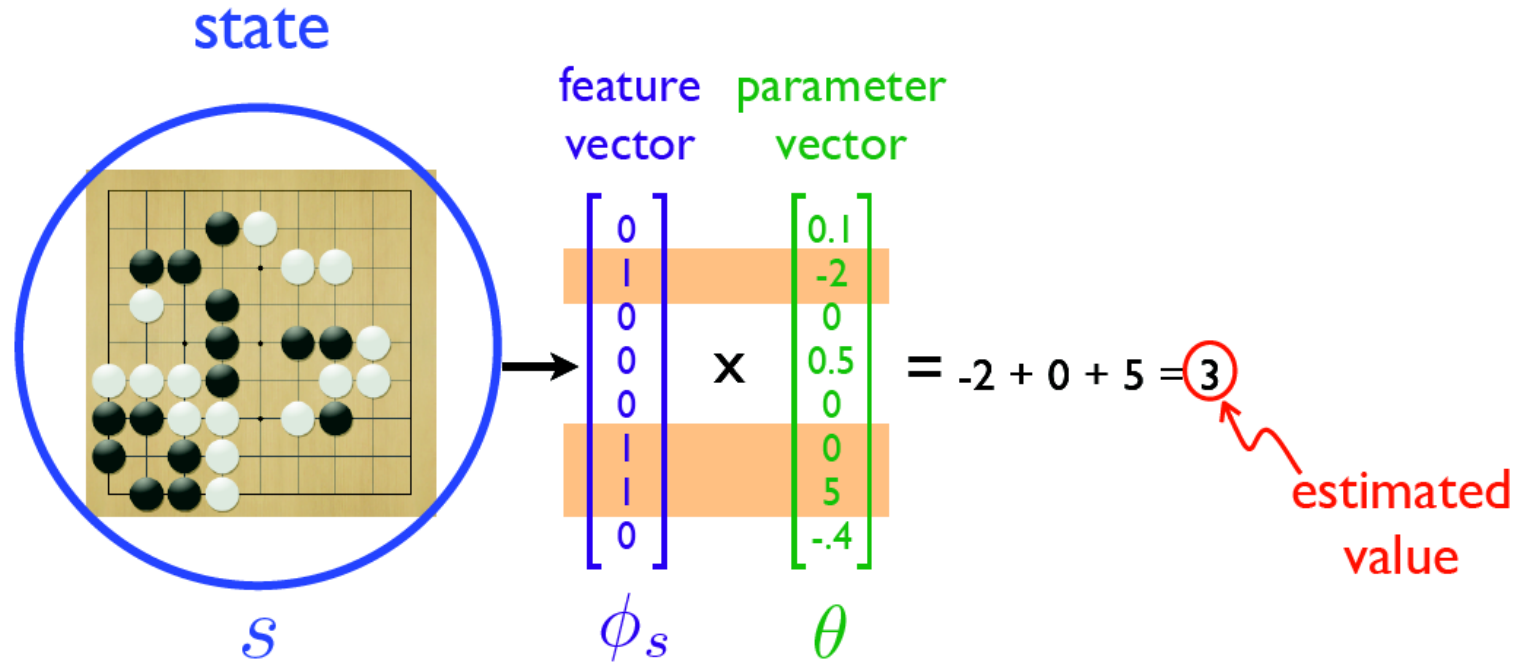
\includegraphics[width=\textwidth]{
		images/19_ReinforcementLearning_functionApproximation.png
	}
	\caption{State utility function approximation.}
	\label{fig:functionApproximation}
\end{figure}

\subsection{Deep Q-learning}
A refinement of the previous idea is to approximate $U(s)$ and $Q(s,a)$ with a
parametric function and introduce a \textbf{deep neural network} to learn the parameters
(Figure \ref{fig:reinforcementLearningDeep}).

\begin{figure}[H]
	\centering
	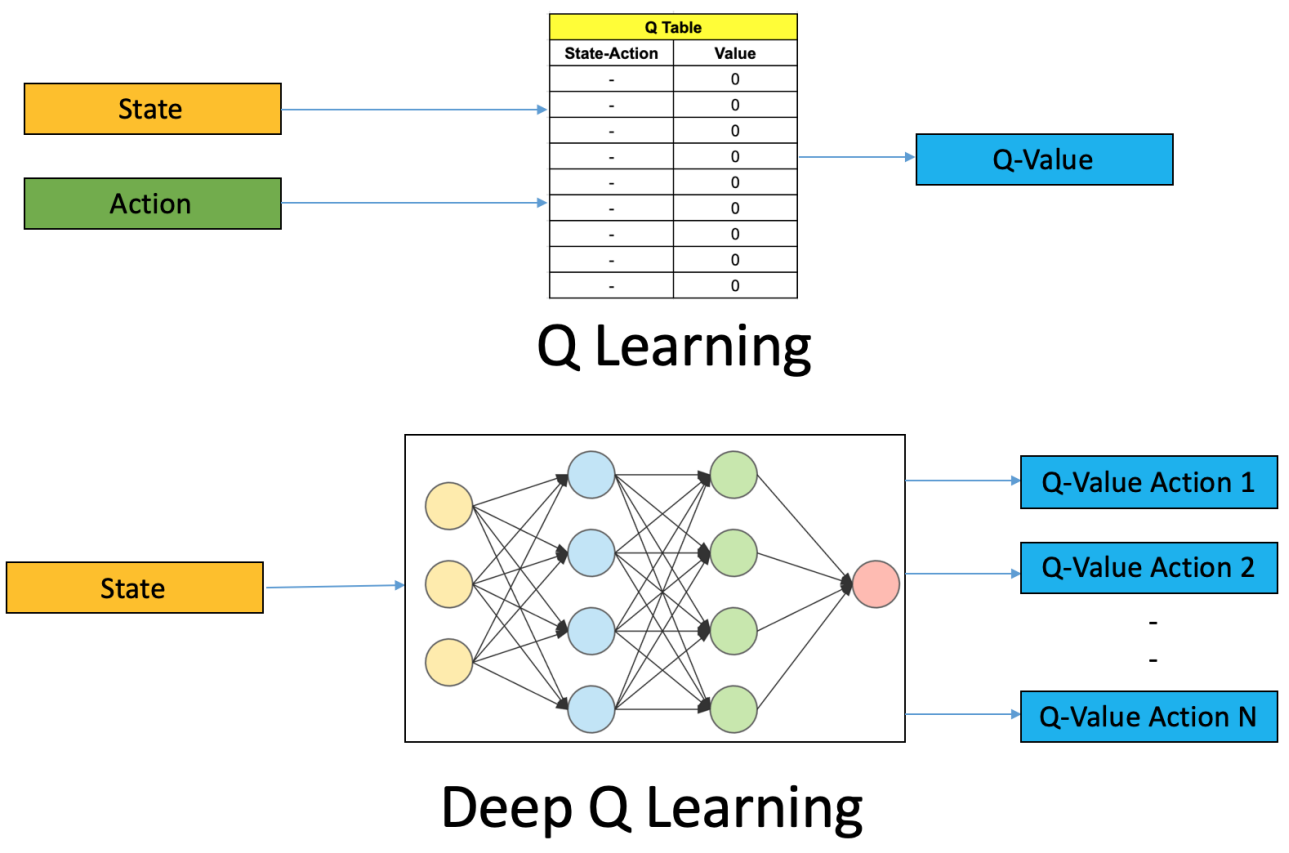
\includegraphics[width=\textwidth]{
		images/19_ReinforcementLearning_deepQLearning.png
	}
	\caption{Q learning and deep Q learning comparison.}
	\label{fig:reinforcementLearningDeep}
\end{figure}

\subsubsection{state utility}
\begin{equation}
	U(s) \approx U_{\theta}(s)
\end{equation}

It is not straightforward to define a proper loss function for this problem. The
professor in the slide writes this formula:

\begin{equation}
	E(s,s') = \frac{1}{2}(R(s) + \gamma U_{\theta}(s') - U_{\theta}(s))^{2}
\end{equation}

This formulation allows us to learn by means of stochastic gradient descent procedure.

\begin{equation}
	\nabla_{\theta}E(s,s') = (R(s) + \gamma U_{\theta}(s') - U_{\theta}(s)) (- \nabla
	_{\theta}U_{\theta}(s))
\end{equation}

In this implementation of stochastic gradient descent, we sample \textit{experiences}
$(s,a,s')$ instead of training set examples.
\newline

The stochastic gradient update rule is:
\begin{equation}
	\theta = \theta - \alpha \nabla_{\theta}E(s, s')
\end{equation}

\subsubsection{action utility}
\begin{equation}
	Q(s,a) \approx Q(s,a)_{\theta}(s)
\end{equation}

It is not straightforward to define a proper loss function for this problem. The
professor in the slide writes this formula:

\begin{equation}
	E((s,a),s') = \frac{1}{2}(R(s) + \gamma \text{max}_{a' \in \mathcal{A}}Q_{\theta}
	(s', a') - Q_{\theta}(s,a))^{2}
\end{equation}

This formulation allows us to learn by means of stochastic gradient descent procedure.

\begin{equation}
	\nabla_{\theta}E((s,a),s') = (R(s) + \gamma \text{max}_{a' \in \mathcal{A}}Q_{\theta}
	(s', a') - Q_{\theta}(s,a)) (- \nabla_{\theta}Q_{\theta}(s,a))
\end{equation}

In this implementation of stochastic gradient descent, we sample \textit{experiences}
$(s,a,s')$ instead of training set examples.
\newline

The stochastic gradient update rule is:
\begin{equation}
	\theta = \theta - \alpha \nabla_{\theta}E((s,a), s')
\end{equation}